\documentclass{article}
\usepackage{listings}

\usepackage[utf8]{inputenc}
\usepackage{amssymb}
\usepackage{lipsum}
\usepackage{amsmath}
\usepackage{fancyhdr}
\usepackage{geometry}
\usepackage{scrextend}
\usepackage[english,german]{babel}
\usepackage{titling}
\setlength{\droptitle}{-3cm}
\usepackage{tikz}
\usepackage{algorithm,algpseudocode}
\usepackage[doublespacing]{setspace}
\usetikzlibrary{datavisualization}
\usetikzlibrary{datavisualization.formats.functions}
\usepackage{polynom}
\usepackage{amsmath}
\usepackage{gauss}
\usepackage{tkz-euclide}
\usetikzlibrary{datavisualization}
\usetikzlibrary{datavisualization.formats.functions}
\title{Übungsblatt 5}
\author{
Alexander Mattick Kennung: qi69dube\\
Kapitel 1
}
\usepackage{import}
\date{\today}
\geometry{a4paper, margin=2cm}
\usepackage{stackengine}
\parskip 1em
\newcommand\stackequal[2]{%
  \mathrel{\stackunder[2pt]{\stackon[4pt]{=}{$\scriptscriptstyle#1$}}{%
  $\scriptscriptstyle#2$}}
 }
\makeatletter
\renewcommand*\env@matrix[1][*\c@MaxMatrixCols c]{%
  \hskip -\arraycolsep
  \let\@ifnextchar\new@ifnextchar
  \array{#1}}
\makeatother
\lstset{
  language=haskell,
}
\lstnewenvironment{code}{\lstset{language=Haskell,basicstyle=\small}}{}
\usepackage{minted}
\usepackage{enumitem}
\setlist{nosep}
\usepackage{titlesec}

\titlespacing*{\subsection}{0pt}{2pt}{3pt}
\titlespacing*{\section}{0pt}{0pt}{5pt}
\titlespacing*{\subsubsection}{0pt}{1pt}{2pt}



\begin{document}
	\maketitle
	Kontakt:\\
	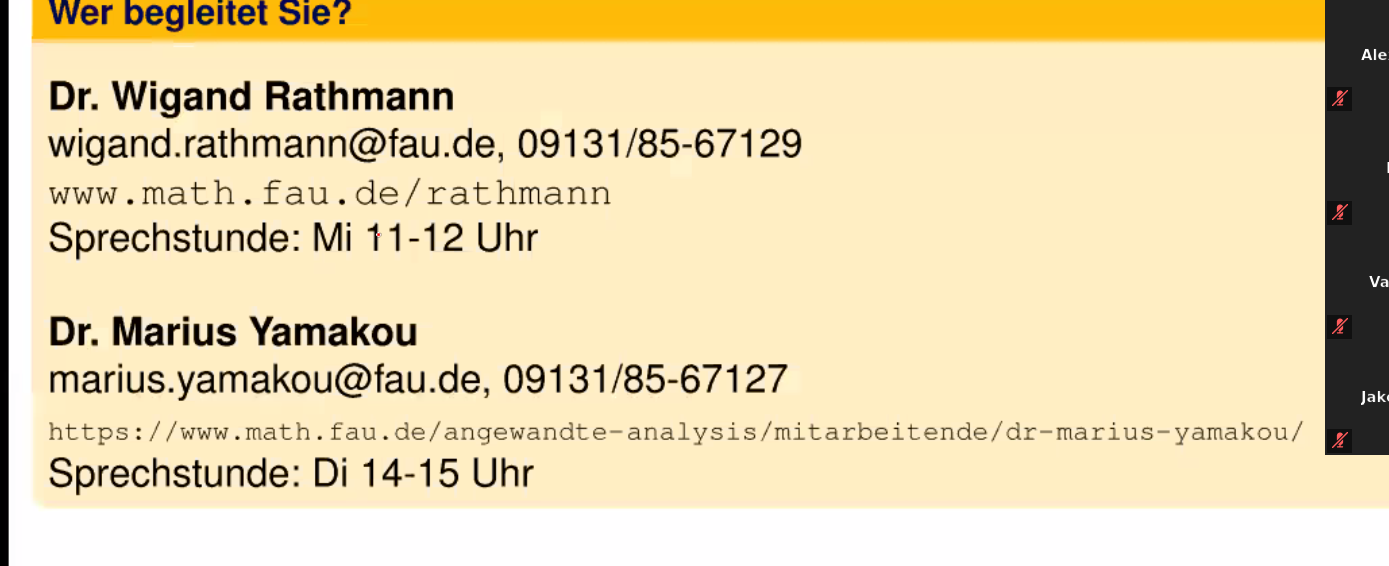
\includegraphics[width=256pt]{Bildschirmfoto_2020-04-20_12-18-32.png}
	\section{Daten und beschreibende Statistik:}
	Kurspasswort: \textbf{Kovarianzmatrix}\\
	\textbf{Ausgabe}: Do/FR vor der ersten Übung, erste am 27.04-30.4\\
	\textbf{Abgabe} de Übungsblätter: \textbf{DO bis 12:00} auf studon, am 7.5 abgabeschluss\\
	Freitag ist ``Fragestunde''\\
	\begin{itemize}
		\item Summe, Produkt
		\item (mehrdimensionale) Riemann-Integration
		\item Abbildungen (vom Ereignis in den Wertraum)
	\end{itemize}
	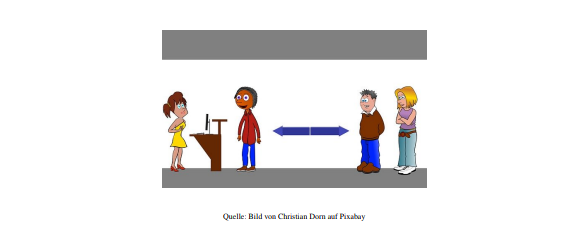
\includegraphics[width=256pt]{warteschlange.png}\\
	Aufteilen der Zeit in diskrete Zeitabschnitte, in jedem Abschnitt gibt es eine chance das ein ereignis X passiert oder nach Y Zeitabschnitte X passiert ist.\\
	\begin{itemize}
		\item nominal: anzahl stunden (nicht vergleichbar)
		\item ordinal: geschlecht (vergleichbar)
		\item metric: ``zufriedenheit'' (vergleichbar, kontinuierliche)
	\end{itemize}
	\textbf{Urliste}\\
	Die Liste aller möglichen daten (zugrundeliegende Verteilung)
	mit Zahlen arbeiten:
	\begin{itemize}
		\item Sortieren
		\item Gruppieren
		\item Kennzahlen
		\item empirsche Verteilungsfunk.
		\item Visualisieren(Histogram, boxplot)
	\end{itemize}
	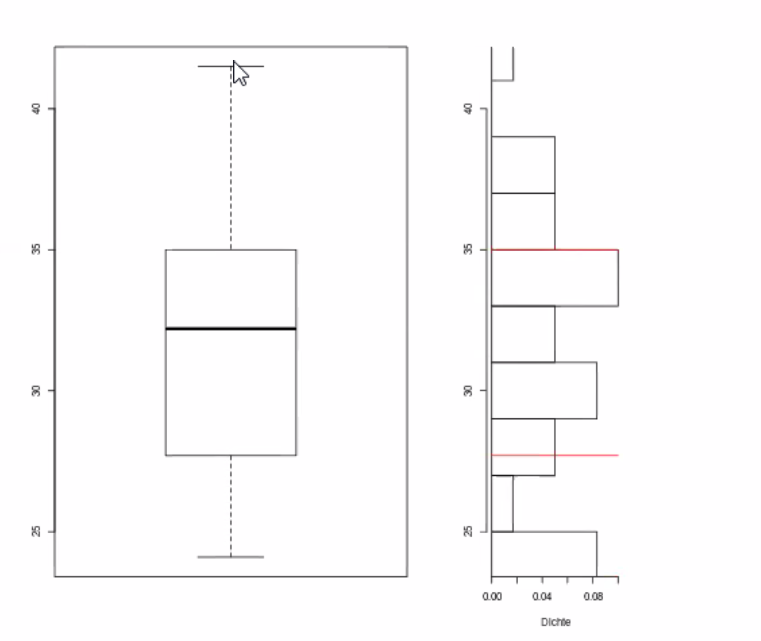
\includegraphics[width=256pt]{Boxplot.png}\\
	Zeigt varianz auf.\\
	Bivariate daten: Zusammenhänge zwischen (zwei) Datensätzen.\\
	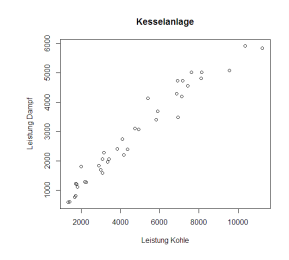
\includegraphics[width=256pt]{bivariat.png}\\
	z.B. lineare Regression\\
	Nach normalisierung sieht man, das der Median nicht gleich ist, also keine linearer zusammenhang sein kann.
	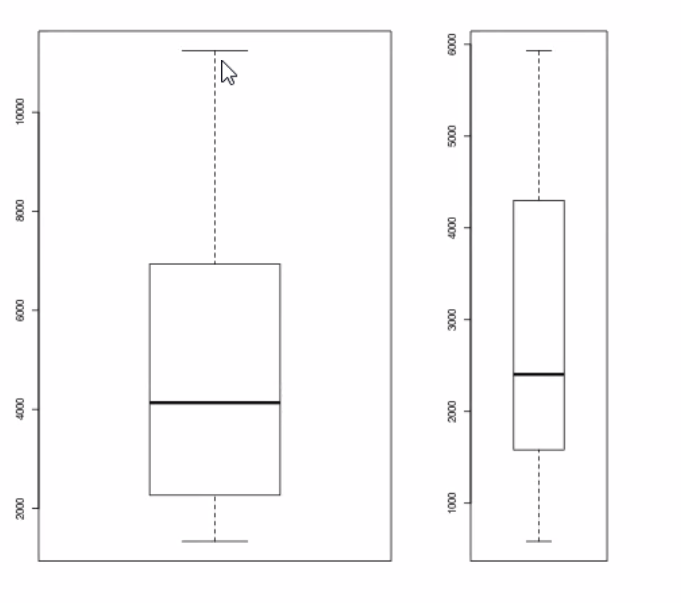
\includegraphics[width=256pt]{kohle.png}\\
	Quantile-Quantile Graph\\
	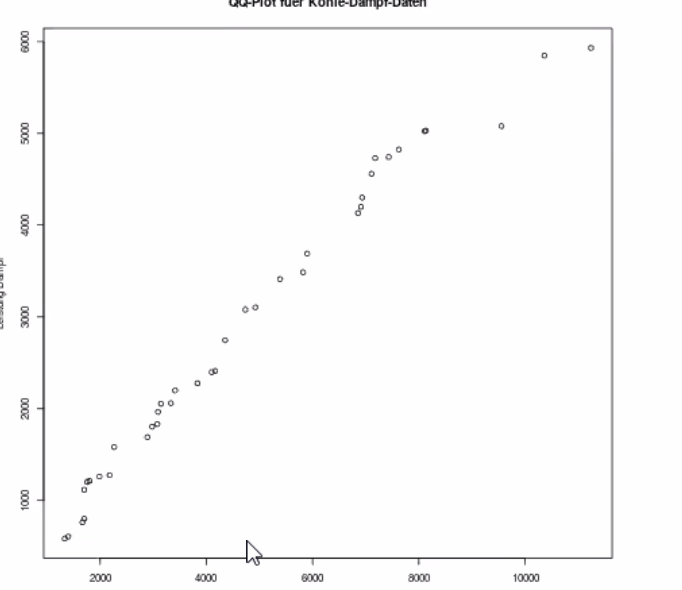
\includegraphics[width=256pt]{QQ-plot.png}\\
	Aufschreiben der nach der größe sortierten werte. In einem perfekten zusammenhang würden beide linear verlaufen.\\
	\begin{itemize}
		\item Zufallsexperiment und Wahrsch. Räume (Vektor/Ereignisraum für Mengen)
		\item Laplace-Exp, Kombinatorik
		\item Bedingte-wahrscheinlichkeit
		\item Wahrsch auf diskreten Mengen (abzählbar)
		\item Verteilung und Zufallsvariablen (Eigentlich keine Variable sondern \textbf{Abbildung})
		\item Erwartungswert/Varianz
		\item Normalverteilung
		\item Mathematische statistik (vorerst beschreibende Statistik, beantworte die Frage: Folgt dieser Stichproben-Urraum einer z.B. normalverteilung)
		\item Grenzwerte
	\end{itemize}
	TODO: \textbf{Ordnungsstatistik,
Rangwert, Mittelwerte, Median, Perzentile, Klassen, empirische Varianz, Standardabweichung, Kovarianz etc.\\
und graphischen Möglichkeiten vertraut (Histogramm, Boxplot,
empirische Verteilungsfunktion)}
	\subsection{Ordnungsstatistik}
	Die Wahrscheinlichkeit der Werte sortiert nach Wert:\\
	Bsp.: Es wurde gemessen $\{6,9,3,8\}$ dann ist die dazugehörige Ordnungsstatistik:\\
	$x_{(1)}=3, x_{(2)}=6,x_{(3)}=8,x_{(4)}=9$ Es gilt also:\\
	$\forall n. x_{(n)}<x_{(n+1)}$ Wobei $x_{(n)}$ der Wert der Messung ist. \textbf{NICHT} deren wahrscheinlichkeit, mehrfach auftauchende Ergebnisse werden mehrfach aufgezählt! Daraus folgt, dass das Minum der Messung $x_{(1)}$ und das Maximum $x_{(n)}$ ist. Die Wertspannweite (nützlich für z.B. normalisierung) ist $x_{(n)}-x_{(1)}$\\
	\subsection{Rang}
	Eine weiter davon induzierte Metrik ist der Rang i: Dies ist einfach der Index der Messung mit diesem Wert. Im Beispiel von oben wäre der Rangwert von $3=x_{(1)}\implies$ Rangwert 1. Der Rangwert ist nicht wohldefiniert, da bei der Messung $\{1,2,3,2,4\}$ Der Rangwert von 2 entweder 2 oder 3 sein kann: $(x_{(1)}=1,x_{(2)}=2,x_{(3)}=2,x_{(4)}=3,x_{(5)}=4)$. In diesem Fall gilt, dass der Rangwert über die s schritte Normalisiert wird: $R(x_{[j]}) = \frac{r+(r+1)+\dots+(r+s-1)}{s}= r+ \frac{s-1}{2}$ Dies wird auch als ``Bindung'' bezeichnet.\\
	\subsection{Klassen}
	Eine Messung wird in eine Klasse aufgrund eines bestimmten Merkmals gepackt (z.B. ``ist Männlich'' oder ``alter$<25$''). Diese Klassen müssen den Raum dicht und überlappungsfrei aufteilen, wobei gilt, dass Klassengruppen durch eine Untere und obere Schranke eindeutig klassifiziert werden können müssen. Somit erhält man einen Spezialfall der Äquivalenzklassen, in der alle Klassen stetig aufgereit sind.
	Formal heißt dies:\\
	sei $x = (x_1,\dots,x_n)$ eine Stichprobe. Diese wird zu l Klassen $K_i,1\leq i\leq l$ zusammengefasst. Dies wird über Grenzpunkte [a,b) bewerkstelligt, für die gilt:\\
	$a=z_0\leq\dots\leq z_l=b$. Somit ist
	\[K_i = (z_{i-1}, z_i]\]
	Die Klasenmitte ist definiert als 
	\[m_i = \frac{z_{i-1}+z_i}{2}\]
	und die relative häufigkeit der Klasse $K_i$ ist
	\[h_i=\frac{|\{j|x_j\in K_i\}|}{n}\]
	
	\subsection{Mittelwerte, Perzentile/Quantile und Median}
	Der Mittelwert ist rein Formal eine funktion von einer Menge M zu einem Wert w.\\
	In der Statistik wird aber häufig das arithmetische Mittel gemeint: 
	\[\overline{x} = \frac{1}{n}\sum\limits^n_{i=1} x_1\]
	wobei n die Mächtigkeit der Menge ist.\\
	Das p-Quantil/Perzentil beschreibt die Anzahl der Werte deren Wahrscheinlichkeit kleiner als p ist:\\
	Sei $X=\{1,3,2,6,3\}$ eine Stichprobe, dann kann aus dieser eine Ordnungsstatistik:\\
	$O=(1,2,3,3,6)$ gebildet werden, mit $o_n\leq o_{n+1}, o_n\in O$.\\
	Das 0.2-Quantil wäre hier der Wert $i=\lfloor 0.2|O|\rfloor$ also $i=\lfloor0.2*5\rfloor=1$
	also ist das 0.2-Quantil gleich $x_{(1)}=1$\\
	Der Unterschied zwischen Perzentil und Quantil ist, dass ein Perzentil in Prozent angegeben wird: das 0.2-Quantil ist das 20-Perzentil.\\
	Man kann das Quantil auch auf kontinuierliche Verteilungen erweitern, solange entweder eine stetige Wahrscheinlichkeitsfunktion F existiert (in diesem Fall $F(x_p)=p$ für ein Quantil p auflösen) oder eine Wahrscheinlichkeitsdichtefunktion f existiert. Dann gilt $\int\limits^{x_p}_{-\infty} f(x)dx = p$ für ein quantil p.\\
	Der median ist das 0.5-Quantil.\\
	\subsection{Varianz, Standardabweichung und empirische Varianz}
	Varianz:\\
	\[\sigma^2 = \frac{1}{N}\sum\limits^N_{i=1} (x_i-\mu)^2\] wobei $\mu$ das arithmetisch mittel ist.\\
	Alternativ wird manchmal für empirsche Varianz durch die Anzahl der Freiheitsgrade geteilt:\\
	\[s^2=\frac{1}{n-1}\sum^n_{i=1} (x_i-\overline{x})^2\]
	Formal muss außerdem beachted werden, dass man bei der empirischen Varianz mit Stichproben arbeitet. Deshalb erhält man nicht den Echten mittelwert $\mu$, sondern nur den Mittelwert der Messung$\overline{x}$.\\
	Alternativ muss u.u. für kontinuierliche Werte ein integral gebildet werden, statt diskret zu summieren!
	Die standardabweichung std ist $\sigma$ bzw die Wurzel der Varianz. Die Varianz ist das Zentrale Moment zweiter Ordnung.
	Das problem mit der Varianz selbst, ist das die Einheit anders als die der Zufallsvariablen ist. Dies ist schon an ihrer Definition sichtbar: Sie ist die (u.u. diskrete) Summe der Abweichungen vom Mittelwert, also erhält man eine summe aus gewichteten Werten, was eine ``Fläche'' darstellt (kleine Scheiben werden zu einer Fläche addiert!). Somit erhält man eine Einheit die die Form (Einheit der Zufallsvariable)$^2$.\\
	Somit ist die Varianz in der Praxis einfacher verwendbar als das zentrale zweite Moment.
	\subsection{kovarianz}
	Die kovarianz gibt an, wie zwei Werte miteinander korrelieren. (Notiz: korrelation ist technisch gesehen die standardisierte kovarianz)
	Eine positive kovarianz sagt aus, dass wenn ein Wert steigt, dann der andere auch steigt, während ein negativer Wert aussagt, dass der eine Wert fällt, wenn der andere steigt. Eine kovarianz von 0 sagt aus, dass zwei worte nicht miteinander zusammenhängen.\\
	\[Cov(x,y) = \frac{1}{N-1}\sum\limits^N_{i=1} (x_i-\overline{x})(y_i-\overline{y})\]
	Das $N-1$ entsteht durch die sogenannte ``Bessler-Korrektur'' und beschreibt die \textbf{Stichprobenkovarianz}, wenn das -1 nicht vorliegt spricht man von der \textbf{Populationskovarianz} (ähnlich zur standardabweichung).
	Die Populationskovarianz kann deshalb auch als
	\[Cov(X,Y) := \mathbb{E}[(X-\mathbb{E}(X)\cdot(Y-\mathbb{E}(Y)))]\]
	Daraus kann man auch sehen, dass X und Y zwei reelle und INTEGRIERBARE zufallsvariable sein müssen.\\
	Die Kovarianz ist symmetrisch in ihren argumenten und sehr sensible gegen outliers!
	\subsection{Histogram}
	Ein Histogram Teilt eine Messungen in (verschieden große) Klassen auf. Die Breite ist abhängig von der größe der Klasse, während der Flächeninhalt die Häufigkeit darstellt.
	Die höhe des Rechtecks stellt dann die Häufigkeitsdichte dar (also die Häufigkeit normalisiert mit der Klassengröße, damit die Werte vergleichbar bleiben)\\




\end{document}